\chapter{Các kiến thức liên quan}

\section{Tổng quan về trải nghiệm du lịch văn hóa và lịch sử tại Việt Nam}
Du lịch văn hóa là một trong những hình thức du lịch đã xuất hiện từ lâu, không
chỉ ở riêng Việt Nam mà còn ở trên thế giới. Nó vẫn luôn là một trong những loại
hình phát triển bậc nhất, giữa vô vàn các loại hình mới như du lịch nghỉ dưỡng, du
lịch sinh thái, du lịch mạo hiểm, …

Du lịch văn hóa là sự di chuyển của con người đến các điểm du lịch văn hóa ở
các quốc gia hay vùng miền không phải nơi họ sống, với mục đích khám phá, mở
rộng kiến thức, kinh nghiệm về nhu cầu văn hóa của họ. Tồn tại ở dạng một loại hình
du lịch của ngành du lịch, và cũng là một ngành kinh doanh có sử dụng các yếu tố
văn hóa như phong tục tập quán, tín ngưỡng, các lễ hội truyền thống, di tích lịch sử,
những kiến trúc, nghệ thuật và các sản phẩm văn hóa khác. Nói cách khác, du lịch
văn hóa cũng là sự khai thác các tài nguyên du lịch văn hóa bao gồm những di tích
lịch sử - văn hóa, công trình kiến trúc nghệ thuật, di tích cách mạng, các giá trị văn
hóa dân gian, lễ hội truyền thống, các công trình lao động sáng tạo của con người,
hoặc khai thác các yếu tố văn hóa tâm linh làm cơ sở và mục tiêu đáp ứng nhu cầu
tâm linh của con người.

Việt Nam ta có lượng tài nguyên du lịch văn hóa dồi dào, thể hiện tiềm năng
phát triển vượt bậc của du lịch văn hóa. Hơn 4000 năm dựng nước và giữ nước, 54
dân tộc anh em đã tạo ra các giá trị truyền thống văn hóa đồ sộ. Bên cạnh đó không
thể không kể đến lượng lớn hơn 44000 danh lam thắng cảnh, di tích lịch sử - với hơn
3000 địa danh là di sản cấp quốc gia, hơn 5000 địa danh cấp tỉnh và 7 di sản văn hóa
được UNESCO công nhận là di sản văn hóa thế giới, cùng 117 bảo tàng và 8000 lễ
hội \cite{huong2022}.

Những con số kể trên phần nào cũng đã thể hiện được ý nghĩa và tầm quan trọng
của du lịch văn hóa. Không chỉ mang về nguồn thu ngân sách khổng lồ với vai trò là
một ngành kinh doanh, nó cũng mang lại những giá trị to lớn về mặt duy trì và bảo
tồn văn hóa.

Về phân loại, ta có thể chia nhỏ các hình thức du lịch văn hóa làm 3 loại hình
nhỏ \cite{vinpearl2022}:

\textbf{Văn hóa vật thể}: Các sản phẩm văn hóa như tranh ảnh, nghệ thuật, dụng cụ,
văn học, .. được tạo ra từ hoạt động sinh hoạt, sáng tạo, thiết kế của người dân và có
giá trị mang tính hiện hữu, vật chất.

\textbf{Văn hóa phi vật thể}: Trái với văn hóa vật thể, văn hóa phi vật thể bao gồm các
giá trị văn hóa về mặt tinh thần, những thứ vô hình, không thể nhìn thấy hay cầm nắm
nhưng có thể cảm nhận, cảm thụ, ví như ca dao tục ngữ, các hình thức diễn xướng,
câu chuyện thần thoại, ca hát, làn điệu nghệ thuật…

\textbf{Văn hóa tâm linh}: Du lịch tâm linh phát triển dựa trên cơ sở khai thác các yếu
tố văn hóa tâm linh, đáp ứng nhu cầu tâm linh cho con người. Du lịch tâm linh gồm
các hoạt động du lịch về các giá trị văn hóa vật thể và phi vật thể có gắn với các giá
trị về tín ngưỡng tôn giáo hay các giá trị tinh thần đặc biệt.

\section{Một số ứng dụng công nghệ hỗ trợ tìm hiểu và khám phá các điểm du lịch
văn hóa lịch sử}
Ứng dụng công nghệ thông tin đã và đang là một xu hướng tất yếu\cite{itdr2022} trong tất
cả các ngành nghề cả ở trong nước và trên thế giới. Sự ra đời của các công nghệ tối
tân như trí tuệ nhân tạo AI, điện toán đám mây, Big Data, Blockchain, công nghệ 3D,
công nghệ thực tế ảo và thực tế tăng cường (VR và AR), internet kết nối vạn vật (IoT),
các công nghệ định vị (GIS, GPS, LBS) thúc đẩy sự thay đổi mạnh mẽ ở mọi khía
cạnh của cuộc sống và việc tìm hiểu, khám phá các điểm du lịch văn hóa lịch sử cũng
không phải là ngoại lệ.

Sự hình thành khái niệm mới về du lịch công nghệ - phát triển du lịch dựa trên
hỗ trợ của công nghệ số \cite{traveloka2022} đã cho thấy rất rõ hiện thực này, và thể hiện rằng đây là
một xu hướng vô cùng tích cực, khi các ứng dụng công nghệ đem tới sự phát triển
mạnh mẽ cho việc trải nghiệm văn hóa lịch sử ở cả chiều rộng và chiều sâu \cite{tapchicongthuong2022}. Theo
chiều rộng, các sản phẩm, dịch vụ văn hóa được đa dạng hóa. Cụ thể như với việc
quảng bá và truyền thông các trải nghiệm du lịch văn hóa, các đơn vị nay đã tận dụng
các nền tảng phổ biến như các website, mạng xã hội để có nhiều lựa chọn hơn và chủ
động về cách tiếp cận du khách. Các hình thức quản lý thông tin về văn hóa, du lịch
cũng được cải thiện với các kho dữ liệu lớn được số hóa, lưu trữ lâu dài với các cổng
tra cứu được thiết kế để dễ dàng tìm hiểu và tiếp cận hơn. Việc khai thác và vận hành
các hoạt động du lịch được đổi mới và đa dạng hơn với các công nghệ số, cụ thể là
các công nghệ 3D, VR, AR, cũng được sử dụng rộng rãi với mục đích bảo tồn các di
sản văn hóa. Bên cạnh đó công nghệ cũng giúp các đơn vị phát triển được nhiều hơn các ứng dụng bổ trợ trải nghiệm tham quan, đôi khi có thể thay thế các phần thuyết
minh và hướng dẫn viên tại các điểm du lịch.

Theo chiều sâu, các sản phẩm và dịch vụ sẵn có được nâng cấp và sửa sang hiện
đại hơn nhờ các ứng dụng công nghệ. Sự cần thiết của các nâng cấp này một phần do
các sản phẩm, dịch vụ trải nghiệm văn hóa đã trở nên cũ, cần được tăng khả năng tiếp
cận, hoặc cần được phát triển thành một trải nghiệm khác có giá trị cao hơn.
Một số các công nghệ được sử dụng phổ biến hiện nay có thể kể đến là công nghệ
3D, AR, Web, ứng dụng di động ... Mỗi công nghệ trên đều đã có được những thành
quả vô cùng nổi bật trong nước và trên thế giới. Ví dụ triển khai trên nền tảng Web,
một trong những ví dụ tiêu biểu có thể kể đến chính là trang
trungbayonline.hoangthanhthanglong.vn \cite{hoangthanh2022}. Website này lưu trữ lại các hoạt động
trưng bày tiêu biểu của Hoàng thành Thăng Long – như sự kiện “Triển lãm Lam
Kinh” \cite{lamkinh2022}, “Đại tướng Văn Tiến Dũng – Danh tướng thời đại Hồ Chí Minh”\cite{vantien2022}, “Tiến
lịch đón xuân sang”\cite{tetviet2022}, … với lượng nội dung được trình bày vô cùng đẹp mắt và
hấp dẫn với các khung tranh, ảnh, nội dung đa phương tiện (\figurename~\ref{HTTL}).

\begin{figure}[h]
    \centering
    \includegraphics[width=0.8\textwidth]{figures/HTTL.png} % Thay bằng tên file hình ảnh thực tế
    \caption{Giao diện trang trưng bày online Hoàng thành Thăng Long \cite{hoangthanh2022}}
    \label{HTTL}
\end{figure}

Không chỉ triển lãm, trang web còn cung cấp các tour tham quan 360 độ với
độ chi tiết cao và các tương tác hấp dẫn bao gồm các bảng biểu thông tin, audio thuyết
minh (\figurename~\ref{HTTL_360}), tiêu biểu như tour “Di Tích Lịch Sử Nhà Và Hầm D67” \cite{d67_2022}, “Di
Tích Lịch Sử Hầm Bộ Tổng Tham Mưu” \cite{bttm2022}.

\begin{figure}[h]
    \centering
    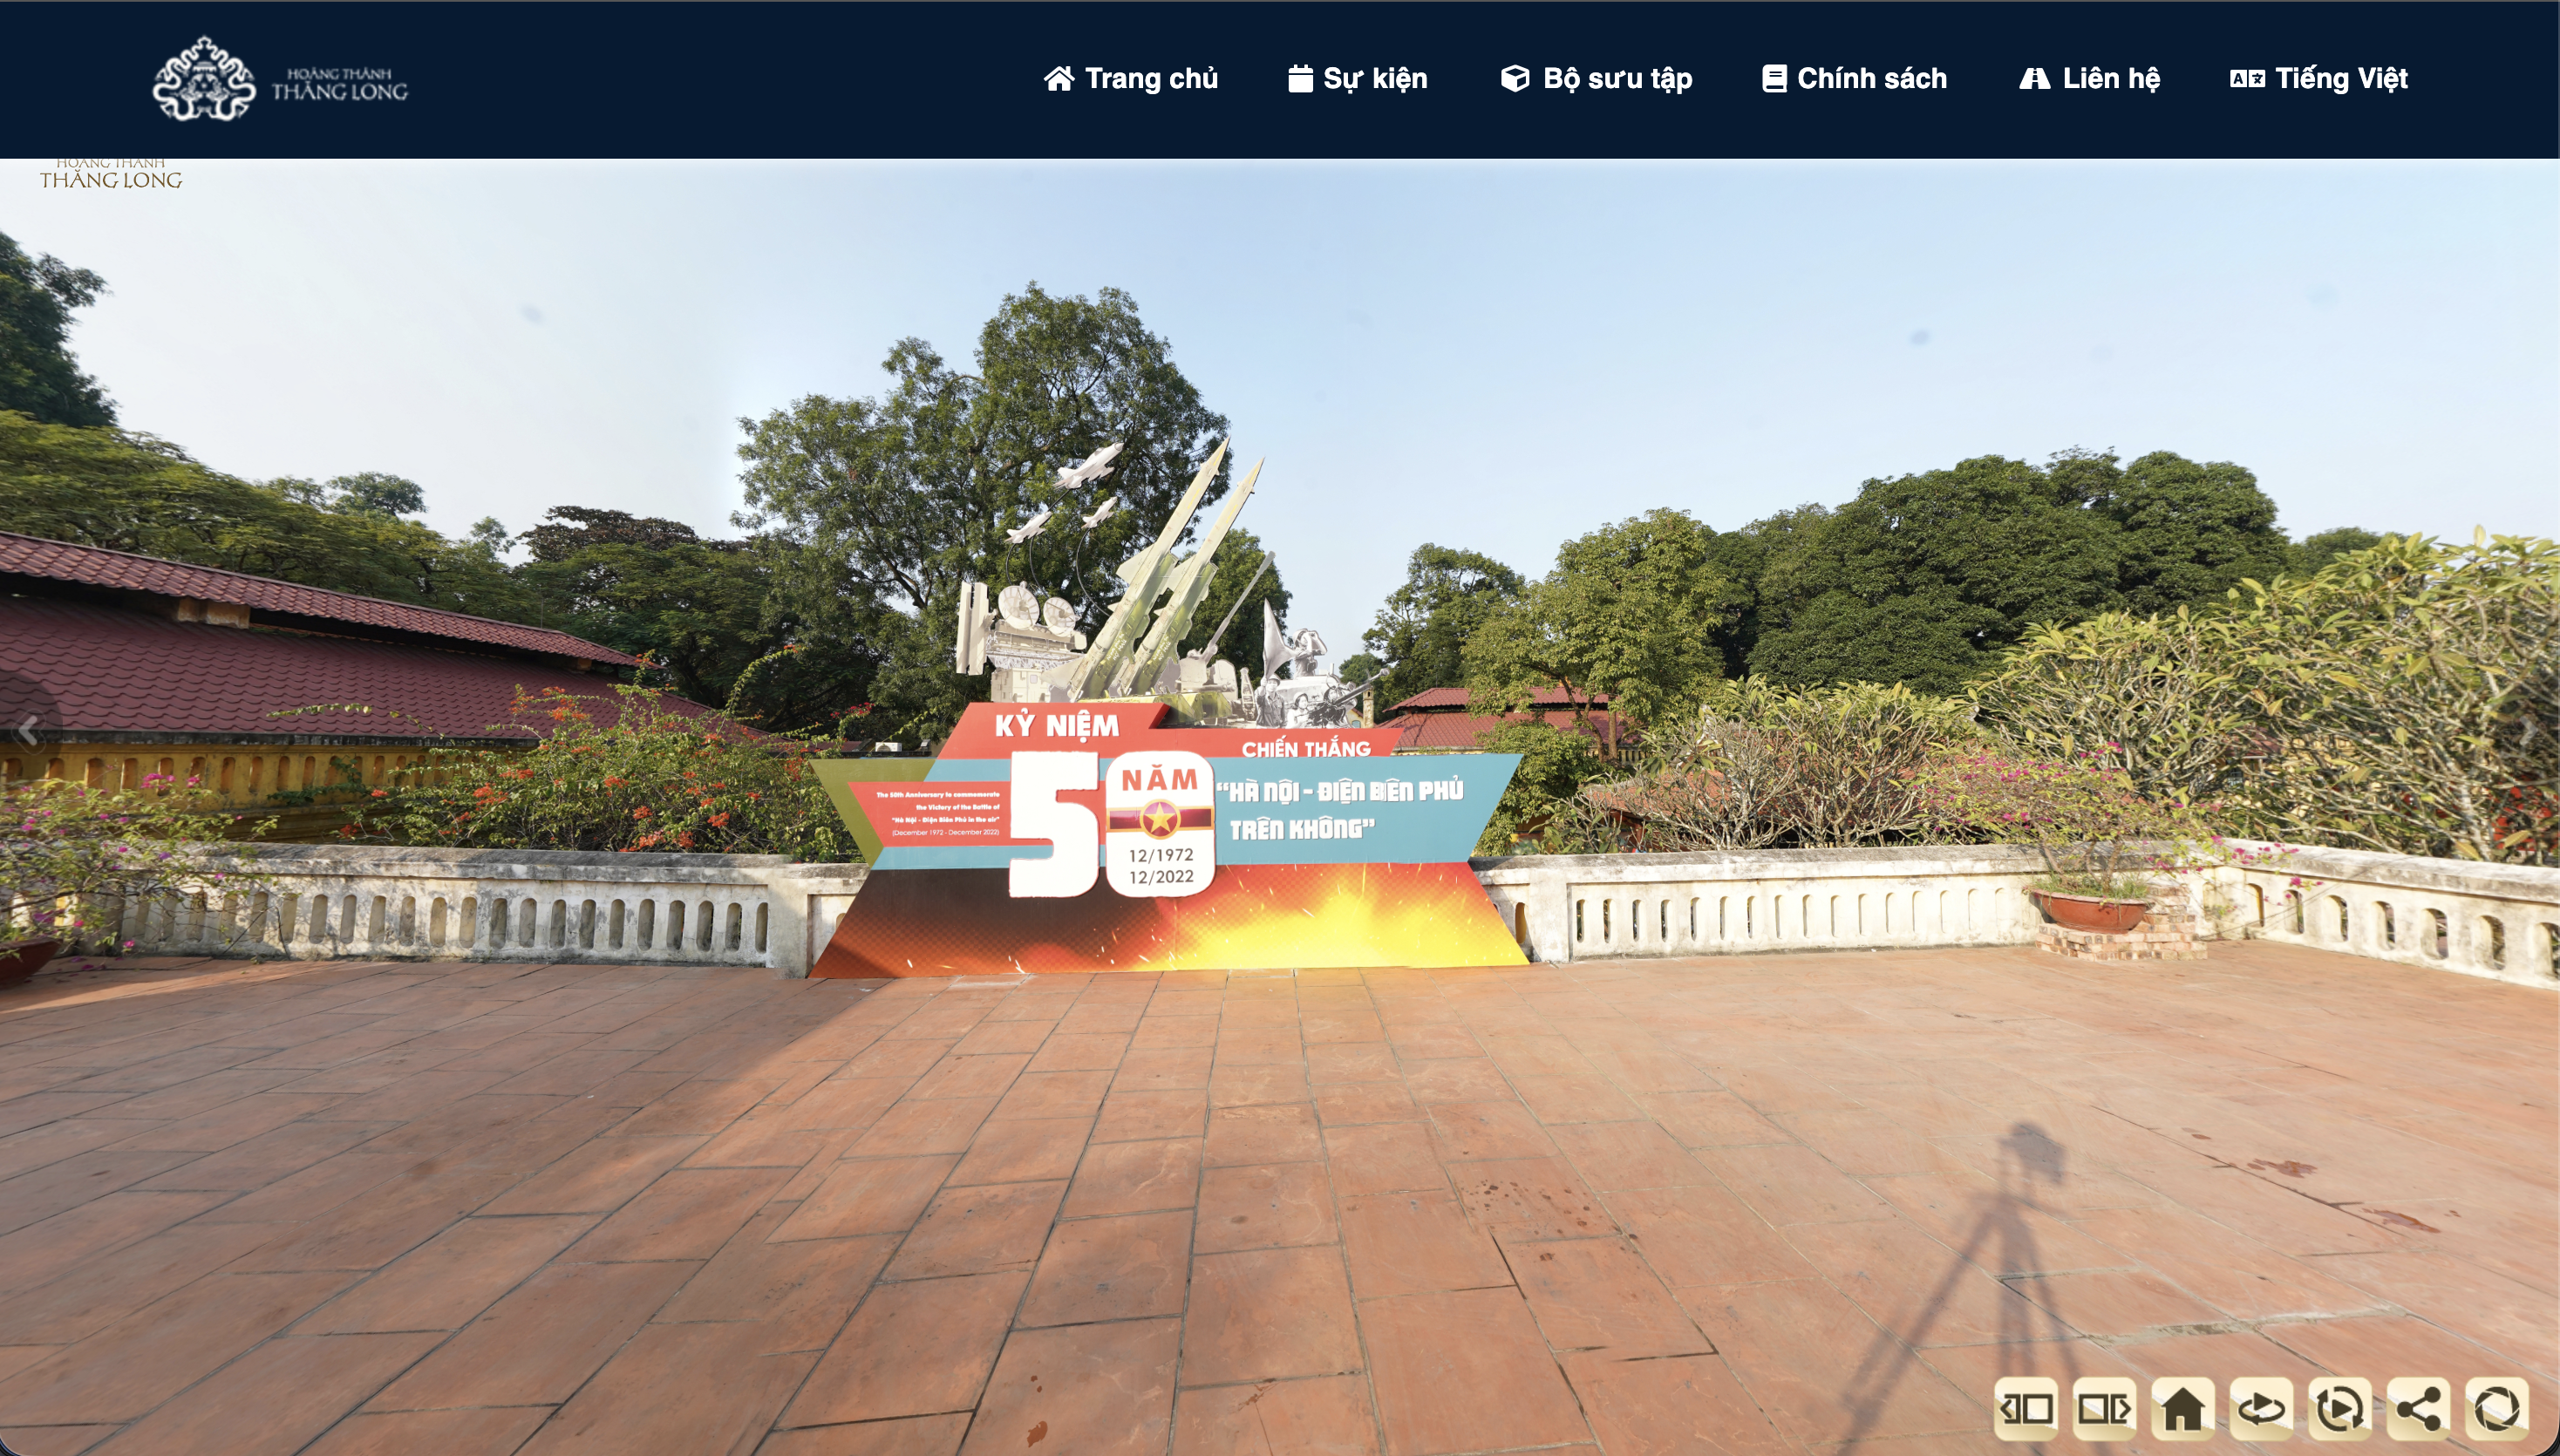
\includegraphics[width=0.8\textwidth]{figures/HTTL_360.png} % Thay bằng tên file hình ảnh thực tế
    \caption{Giao diện tour tham quan 360 độ trên trang trưng bày online Hoàng thành Thăng Long \cite{hoangthanh2022}}
    \label{HTTL_360}
\end{figure}

Với ứng dụng di động, các đơn vị văn hóa như Bảo tàng Lịch sử Quốc Gia
\cite{vtv2022}, Khu di tích Cố đô Huế \cite{hue2022} đều đã triển khai và ứng dụng thành công công nghệ
mã QR trong việc thuyết minh và biểu diễn các điểm tham quan trên thiết bị điện
thoại thông minh. Cung cấp trải nghiệm thuận tiện và đầy đủ thông tin cho du khách,
giúp du khách có thể độc lập trải nghiệm và tìm hiểu điểm tham quan khi không có
hướng dẫn viên.

Nhận thấy việc ứng dụng công nghệ thông tin vào nâng cao trải nghiệm văn
hóa là một nhu cầu hợp lý và cấp thiết, đồng thời hướng đến hỗ trợ du khách và các
đơn vị văn hóa trong việc tạo ra và tham gia vào các trải nghiệm có tính định hướng
cao với nội dung thông tin chính xác, khoá luận vận dụng các công nghệ về bản đồ điện
tử, định vị, ứng dụng web và ứng dụng di động để tạo ra TMAP – một hệ thống bao
gồm phần trình biên soạn – dành cho các đơn vị văn hóa để tạo ra và tùy chỉnh các
bản đồ với các điểm du lịch được định vị và số hóa, mô tả bằng các thông tin đa
phương tiện đa dạng, và cung cấp hình thức tương tác với điểm du lịch đó, phần trình
trải nghiệm – dành cho người dùng phổ thông, các du khách có nhu cầu tham quan
một cách đầy đủ, trọn vẹn, có tuần tự các địa điểm văn hóa, và lưu trữ các tương tác
như hình ảnh, âm thanh, nhận xét của bản thân đối với các địa điểm văn hóa đó.

\section{Cách thức thể hiện dữ liệu dưới dạng TMAP}
Một Map trong TMAP sẽ là một bản đồ chứa các địa điểm tham quan mà
người biên soạn cung cấp cho người dùng. Các điểm tham quan này có thể được tùy
biến trình tự, và mỗi điểm sẽ cho phép người biên soạn cung cấp thông tin mô tả về
điểm du lịch, định hướng trải nghiệm của du khách thông qua hệ thống các tương tác
sẵn có với điểm du lịch.

Ưu điểm của hình thức này đầu tiên là sự chính xác về tính không gian và
thông tin của các điểm du lịch. Du khách sẽ không bị phụ thuộc vào các kết quả có
phần tạp và dễ bị nhầm lẫn của các công cụ tìm kiếm. Bên cạnh đó TMAP mang đến
sự tiện lợi với sự thân thiện dễ sử dụng, và sự tập trung về tính năng.

Với các ưu điểm này của TMAP, em đã lựa chọn để phát triển một hệ thống
kết hợp bao gồm trình biên soạn và trình trải nghiệm. Bộ hai ứng dụng này sẽ tạo ra
môi trường và nền tảng để các nhà biên soạn nội dung kiến trúc nên trải nghiệm đặc
sắc, và đưa đến cho người dùng trải nghiệm đó một cách đơn giản, gần gũi

\section{Công nghệ sử dụng xây dựng TMAP}
